\chapter{Detectors Test, alignment and calibrations.} \label{analysis}
\commento{
\begin{outline}[enumerate]
\1 development of the analysis program.
\1 testing the analysis program with montecarlo data.
\1 Test of the detectors in the Lab.
\1 Beam line description.
\1 Data Analysis
	\2 thresholds scan
	\2 Rates on $Pb^{208}$.
	\2 Beam related asymmetry correction.
	\2 $C^{12}$ Asymmetry.
\end{outline}}

\paragraph{Introduction}
In this chapter we discuss the electronic test that have been carried out in the laboratory, and the calibrations that need to be done
in order to calculate, from the raw data, the final data ready for the analysis.
The test in the lab consist in checking that the photomultipliers are working and that the electronics that take care of acquiring the data do not have any errors.
For the calibrations, since several beam parameters are needed for the analysis, it's importat to obtain the correct scaling factor to convert the Raw Data collected by the \textit{VFC}s to data with the right physical units, as the $X,Y$ impact point of the beam on the target, the beam energy $E$, the beam currer $I$ and the scattering angles $\theta_{x}$ and $\theta_{y}$.

\section{Data tree}
\commento{Explain how we compute all the values for the data tree, the position of the beam on the target, the angle, the correlated-difference values...}

\section{Detectors test}

\commento{Explain the test of the two detectors in the lab, how we select the threshold, the correlation of the pmts and coincidence to select the threshold. Mention also that we observed two knees in the plot of counts vs. attenuation.}

The Nino board, which digitizes the signal from the PMTS, has two parameters which can be used to select the internal threshold of the discriminator, to cut the low amplitude signals and can be adjusted changing the settings of the DAQ program. These two parameters are \textit{Threshold} and \textit{Attenuation}. \textit{Threshold} means directly the charge value necessary for an impulse certain shape to be accepted by the signal discriminators. However the "physical" threshold can be also modified changing the \textit{attenuation}. The relation between threshold and attenuation is not linear, but follows:

\begin{figure}[hbtp]
\centering
\subfloat[][\emph{Threshold dependence against attenuation} \label{NinoDocu}]{
\includegraphics[scale=0.4]{Analysis/ThrvsAtt.png}}
\end{figure}

For our purposes, we select a common threshold values for all the pmts, and we decided to change only the attenuation values.\\
Before the Beam time, some test with the two detectors were performed, to check that the pmts were still working after some years of inactivity, and that the new electronic was able to count properly the pulses and store the data. For this studies, we didn't have a radioactive sources to employ, so we moved the two detectors in the workshop of the accelerator, and we use the cosmic rays rate as a probe. 

Knowing that the expected number of event for cosmic rays is about $1 \frac{event}{\SI{}{\centi \meter\squared} \SI{}{\second}}$ we can compute the expected values for the number of events. We decided to take 1 minute long acquisition for both the two detectors, this leads to $70$ expected events for detector B  and  $100$ events for detector A.  \smallskip

The first step is to select a good point of work for the threshold. So, fixing the value of the threshold parameter for the NINO board, we took several acquisitions, each of them one minute long, increasing each time the attenuation. We powered the pmts with a negative voltage around $ \SI{-1000}{\volt}$, as suggested in the datasheets, and covered the cherenkov detector with a shielding blanket, to avoid ambient light simulating a signal.

\begin{figure}[hbtp]
\centering
\subfloat[][\emph{Attenuation scan for Detector B}]{
\includegraphics[width = 0.45\textwidth]{Analysis/AttenuationB.pdf}}
\subfloat[][\emph{Detector B Counts versus attenuation,the area with constant counts is highlighted }]{
\includegraphics[width = 0.47 \textwidth]{Analysis/AttenuationBlinear.pdf} }
\end{figure}

We observed a small knee in the plot, around the zone of 580 − 600 of attenuation, where the number of counts was almost costant, roughly equal to the number of expected events from muons hitting the detector. Then we observe a big edge for attenuation = 1000. Looking at the plot \ref{NinoDocu}, we assume that the attenuation values are so high that electronic noise is no longer rejected, in fact the counts grow enormously. The attenuation was set at 600.

The next step was to study the statistical fluctuation of the counts, so we collected 10 acquisitions, each of them 1 min long. The measured values are reported in the table below:

\begin{center}
\begin{tabular}{|c|c|c|c|}
\hline 
Pmt: & 1 & 2 & 3 \\ 

1 & 58 & 60 & 62 \\ 
\hline 
2 & 62 & 55 & 59 \\ 
\hline 
3 & 61 & 59 & 70 \\ 
\hline 
4 & 73 & 66 & 70 \\ 
\hline 
5 & 68 & 66 & 56 \\ 
\hline 
6 & 59 & 52 & 64 \\ 
\hline 
7 & 69 & 74 & 77 \\ 
\hline 
8 & 48 & 49 & 57  \\ 
\hline 
9 & 70 & 54 & 58 \\ 
\hline 
10 & 60 & 61 & 66\\
\hline
\end{tabular} 
\end{center}

This data are interesting to check if the counts are following the theoretical distribution of the events expected for cosmic rays at sea level. If the pmt are working in a good mode, we know that the number of counts should be Poisson-distributed:

\begin{equation}
Pdf(\mu,k) =  \frac{\mu^{k}}{k!} e^{-\mu}
\end{equation}

The variance of the poisson distribution is equal to the mean of the counts, and we expect the same behaviour also for the sample mean and the sample variance:

\begin{align*}
\begin{split}
\mu_{1} = 62.8	\qquad \sigma^{2}_{1} = 54.40 \qquad r_{12} = 0.66\\
\mu_{2} = 59.6	\qquad \sigma^{2}_{2} = 57.15 \qquad r_{23} = 0.65\\
\mu_{3} = 63.9	\qquad \sigma^{2}_{3} = 46.98 \qquad r_{13} = 0.35 \\
\end{split}
\end{align*}

We report also the correlation $r_{xy}$ between the pmt. The result are fine: we are able to see a positive correlation between adjacent pmt, and as expected the correlation is lower in the case of the more distant. This is explained by the lower probability that the photons of Cherenkov radiation light up at the same time the more distant pmt.
We can test that the data follow a possion distribution using the well-known Gosset test, defined as:

\begin{equation}
\chi^{2}_{n-1} = \sum_{i = 1}^{n} \dfrac{(Oss_{i} - Att_{i})}{Att_{i}}
\end{equation}

We report the result obtain with the data for detector B, the test shows that there is good agreement with the hypothesis that the count are really poisson-distributed.

\begingroup
\setlength{\tabcolsep}{8pt} % Default value: 6pt
\renewcommand{\arraystretch}{1.2} % Default value: 1
\begin{center}
\begin{tabular}{|c|c|c|c|}
\hline 
Pmt: & 1 & 2 & 3 \\ 
\hline
$\chi^{2}_{9}$ & 8.52 & 8.45 & 6.37 \\ 
\hline
\end{tabular} 
\end{center}
\endgroup

To convince oneself that the pmt are actually measuring signals given by the passage of cosmic rays, and not noise, we exploit the possibility of we exploited the possibility of placing one pmt in coincidence with the others. If we are able to observe correlation between the counts, we can conclude that the detection electronics are working correctly. \\
One pmt was placed over the detector and we read out the counts simultaneously.

\begin{center}
\begin{tabular}{|c|c|c|c|c|}
\hline 
pmt & 0 & 1 & 2 & 4 (in coincidence) \\ 
\hline 
1 & 63 & 57 & 72 & 28 \\ 
\hline 
2 & 55 & 51 & 64 & 18 \\ 
\hline 
3 & 62 & 53 & 75 & 27 \\ 
\hline 
4 & 71 & 62 & 75 & 33 \\ 
\hline 
5 & 68 & 59 & 49 & 23 \\ 
\hline 
6 & 57 & 55 & 63 & 18 \\ 
\hline 
7 & 70 & 64 & 64 & 24 \\ 
\hline 
8 & 50 & 69 & 69 & 25 \\ 
\hline 
9 & 65 & 62 & 62 & 19 \\ 
\hline 
10 & 74 & 71 & 77 & 28 \\ 
\hline 
\end{tabular} 
\end{center} 

As above, we report the sample mean, the variance and the correlation between the pmt in coincidence and the detector B:

\begin{equation*}
\begin{split}
\mu_{0} = 63.5 \qquad \sigma^{2} = 58.9 \qquad r_{04} = 0.49 \\
\mu_{1} = 60.3 \qquad \sigma^{2} = 43.3 \qquad r_{14} = 0.38 \\
\mu_{2} = 67.0 \qquad \sigma^{2} = 71.1 \qquad r_{24} = 0.65 \\
\end{split}
\end{equation*}

We observe a positive correlation $r_{04},r_{14},r_{24}$ for the pmt in coincidence, this is a strong evidence that the signals are correlated and that some particles are hitting the fused silica sequentially. \smallskip

\begingroup
\setlength{\tabcolsep}{8pt} % Default value: 6pt
\renewcommand{\arraystretch}{1.2} % Default value: 1
\begin{center}
\begin{tabular}{|c|c|c|c|c|}
\hline 
Pmt: & 1 & 2 & 3 & pmt in coincidence \\ 
\hline
$\chi^{2}_{9}$ & 8.95 & 6.44 & 10.96 & 9.52\\ 
\hline
\end{tabular} 
\end{center}
\endgroup
\smallskip

We also check at the oscilloscope if we were able to observe three negative peaks at the same time: 

\begin{figure}
\centering
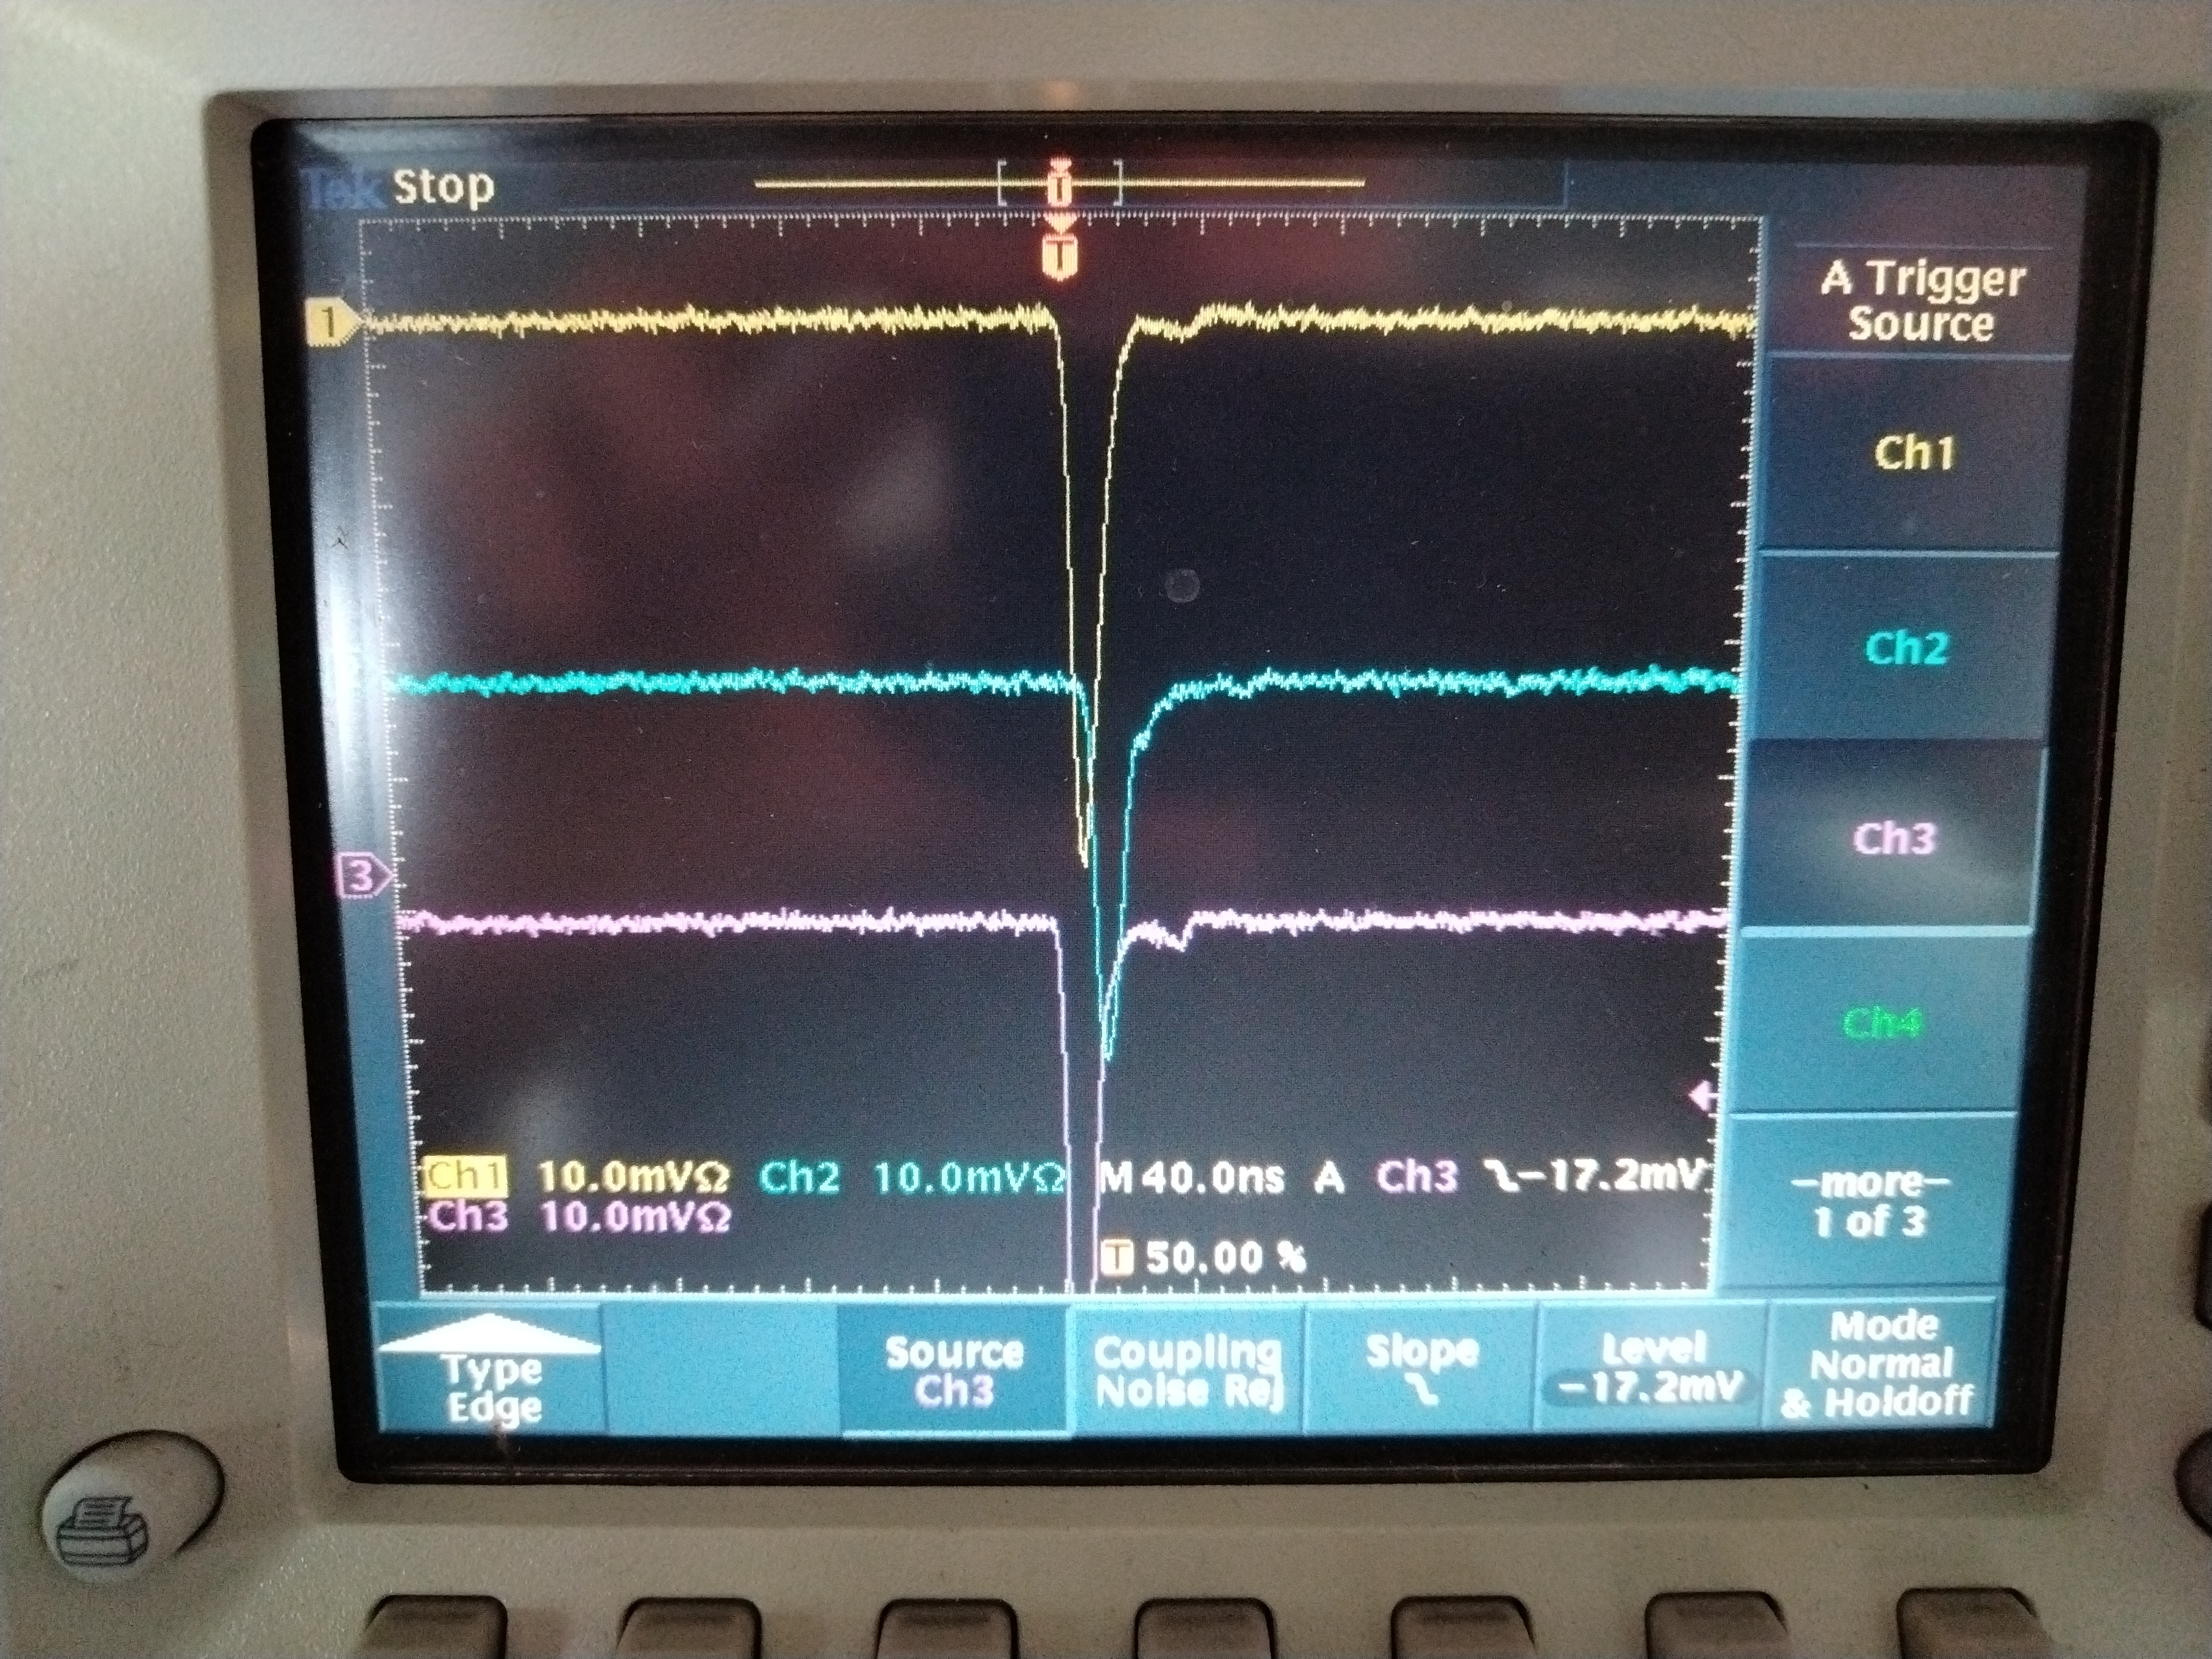
\includegraphics[width = 0.5\textwidth]{Analysis/IMG_20221027_170925.jpg} 
\end{figure}

The same procedure was followed also for detector A, made by 8 PMTs. We analyzed 4 pmt at a time, having the NINO board available with only 4 channels. The same attenuation scan performed for detector B was done:

\newpage
\begin{figure}[hbtp]
\centering
\includegraphics[width = 0.5\textwidth]{Analysis/AttenuationA(4-7).pdf}
\caption{Attenuation scan for Detector A}
\end{figure}

For these 4 pmt we are able to observe 


We took as above 10 acquisitions 1 minute long:

\begin{center}
\begin{tabular}{|c|c|c|c|c|}
\hline 
pmt & 2 & 1 & 0 & 4 (in coincidence) \\ 
\hline 
1 & 91 & 51 & 50 & 27 \\ 
\hline 
2 & 86 & 61 & 50 & 7 \\ 
\hline 
3 & 58 & 48 & 45 & 18 \\ 
\hline 
4 & 95 & 62 & 41 & 29 \\ 
\hline 
5 & 69 & 60 & 50 & 21 \\ 
\hline 
6 & 85 & 57 & 45 & 19 \\ 
\hline 
7 & 66 & 51 & 46 & 28 \\ 
\hline 
8 & 74 & 51 & 48 & 22 \\ 
\hline 
9 & 77 & 43 & 45 & 17 \\ 
\hline 
10 & 62 & 44 & 50 & 29 \\ 
\hline 
\end{tabular} 
\end{center}

\begin{equation*}
\begin{split}
\mu_{2} = 76.3 \qquad \sigma^{2} = 160  \\
\mu_{1} = 52.8 \qquad \sigma^{2} = 47.5 \\
\mu_{0} = 47.0 \qquad \sigma^{2} = 9.6  \\
\mu_{4} = 21.7 \qquad \sigma^{2} = 48.2 \\
\end{split}
\end{equation*}

For these 4 pmts , the variance of the sample changes significantly from what was observed earlier. We repot in this table the correlation matrix:

\begin{center}
\begin{tabular}{|c|c|c|c|c|}
\hline 
pmt: & 4 & 0 & 1 & 2 \\ 
\hline 
4 	 & 1 & -0.18  & -0.21  & -0.06  \\ 
\hline 
0 	 & -0.18  & 1 & -0.10  & -0.22  \\ 
\hline 
1    & -0.21  & -0.10  & 1 & 0.56  \\ 
\hline 
2    & -0.06 & -0.22  & 0.56  & 1 \\ 
\hline 
\end{tabular} 
\end{center}

Here we observe correlation that with negative sign, which are not expected. Also the correlatio between the pmt in coincidence are negative.
If we try to perform a gosset test, we obtain:

\begingroup
\setlength{\tabcolsep}{8pt} % Default value: 6pt
\renewcommand{\arraystretch}{1.2} % Default value: 1
\begin{center}
\begin{tabular}{|c|c|c|c|c|}
\hline 
Pmt: & 2 & 1 & 0 & pmt in coincidence \\ 
\hline
$\chi^{2}_{9}$ & 19.6 & 8.30 & 1.90 & 39.5\\ 
\hline
\end{tabular} 
\end{center}
\endgroup
\smallskip

The expected error for the result of this test is $\sigma = \sqrt{2*(n-1)} \simeq 4$. In this case we are observing 3 values that are $2\cdot \sigma $ far from the expected value. All this consideration indicate that the attenuation, or something in the DAQ program is not correctly set. 

\section{Calibrations.}

One of the main goal for this experiment was to measure the well know trasverse asymmetry of $^{12}C$, already measured before, as a test for the new electronic system. Previous measurements of the Transverse asymmetry have been performed for a carbon target. For this beam-time, the two spektrometers were placed at an angle such that the $Q^{2}$ values of the scattered electron is:

\begin{flushleft}
\begin{align*}
& Spektrometer A : \qquad Q^{2} = \SI{0.041337}{\giga \electronvolt} \qquad \textnormal{without Cut} \\
& Spektrometer A : \qquad Q^{2} = \SI{0.0394513}{\giga \electronvolt} \qquad \textnormal{with Cut} \\
& Spektrometer B : \qquad Q^{2} = \SI{0.0404771}{\giga \electronvolt} \qquad \textnormal{without Cut} \\
& Spektrometer B : \qquad Q^{2} = \SI{0.0405843}{\giga \electronvolt} \qquad \textnormal{with Cut} 
\end{align*} 
\end{flushleft}

The $Q^{2}$ values is the same of the last measurement performed at MAMI, and is measured with and without rejecting the inelastic electrons. 



\subsection{Alignment of the scattering plane}

\subsection{Calibration of the VFCs monitors}
\commento{Maybe it's important to divide this sections in two different part: the first part where I explain the Vfc convert the input voltage signal to a digital signal. In the second part just mention how we tuned the resistences (for X,Y monitors directly at the output signal with the oscilloscope, while for I21 and I13 monitors we used the data, so I'm able to produce plots only for the second ones).}

\subsection{Calibration of the PIMO monitors}

For the calibration of the X Y monitors, we used two target made by three carbon wires at a certain distance from each other, aligned horizontaly and vertically. The distance between the two center of the external wires is $ d_{horizontal} = \SI{2.38}{\milli \meter}$ for the target alligned horizontally and $d_{vertical} = \SI{2.33}{\milli \meter}$ for the other one.
When the horizontal wires target is cetered, we turn on the beam, and we take some data slowly changing the horizontal beam direction. The beam direction is changed by MAMI operators, varying the Magnetic field of the \textit{Wobbler 16} magnets (\ref{fig:BeamLine}):

\begin{wrapfigure}{r}{0.4\textwidth}
%\setlength{\columnsep}{10pt}%
\centering
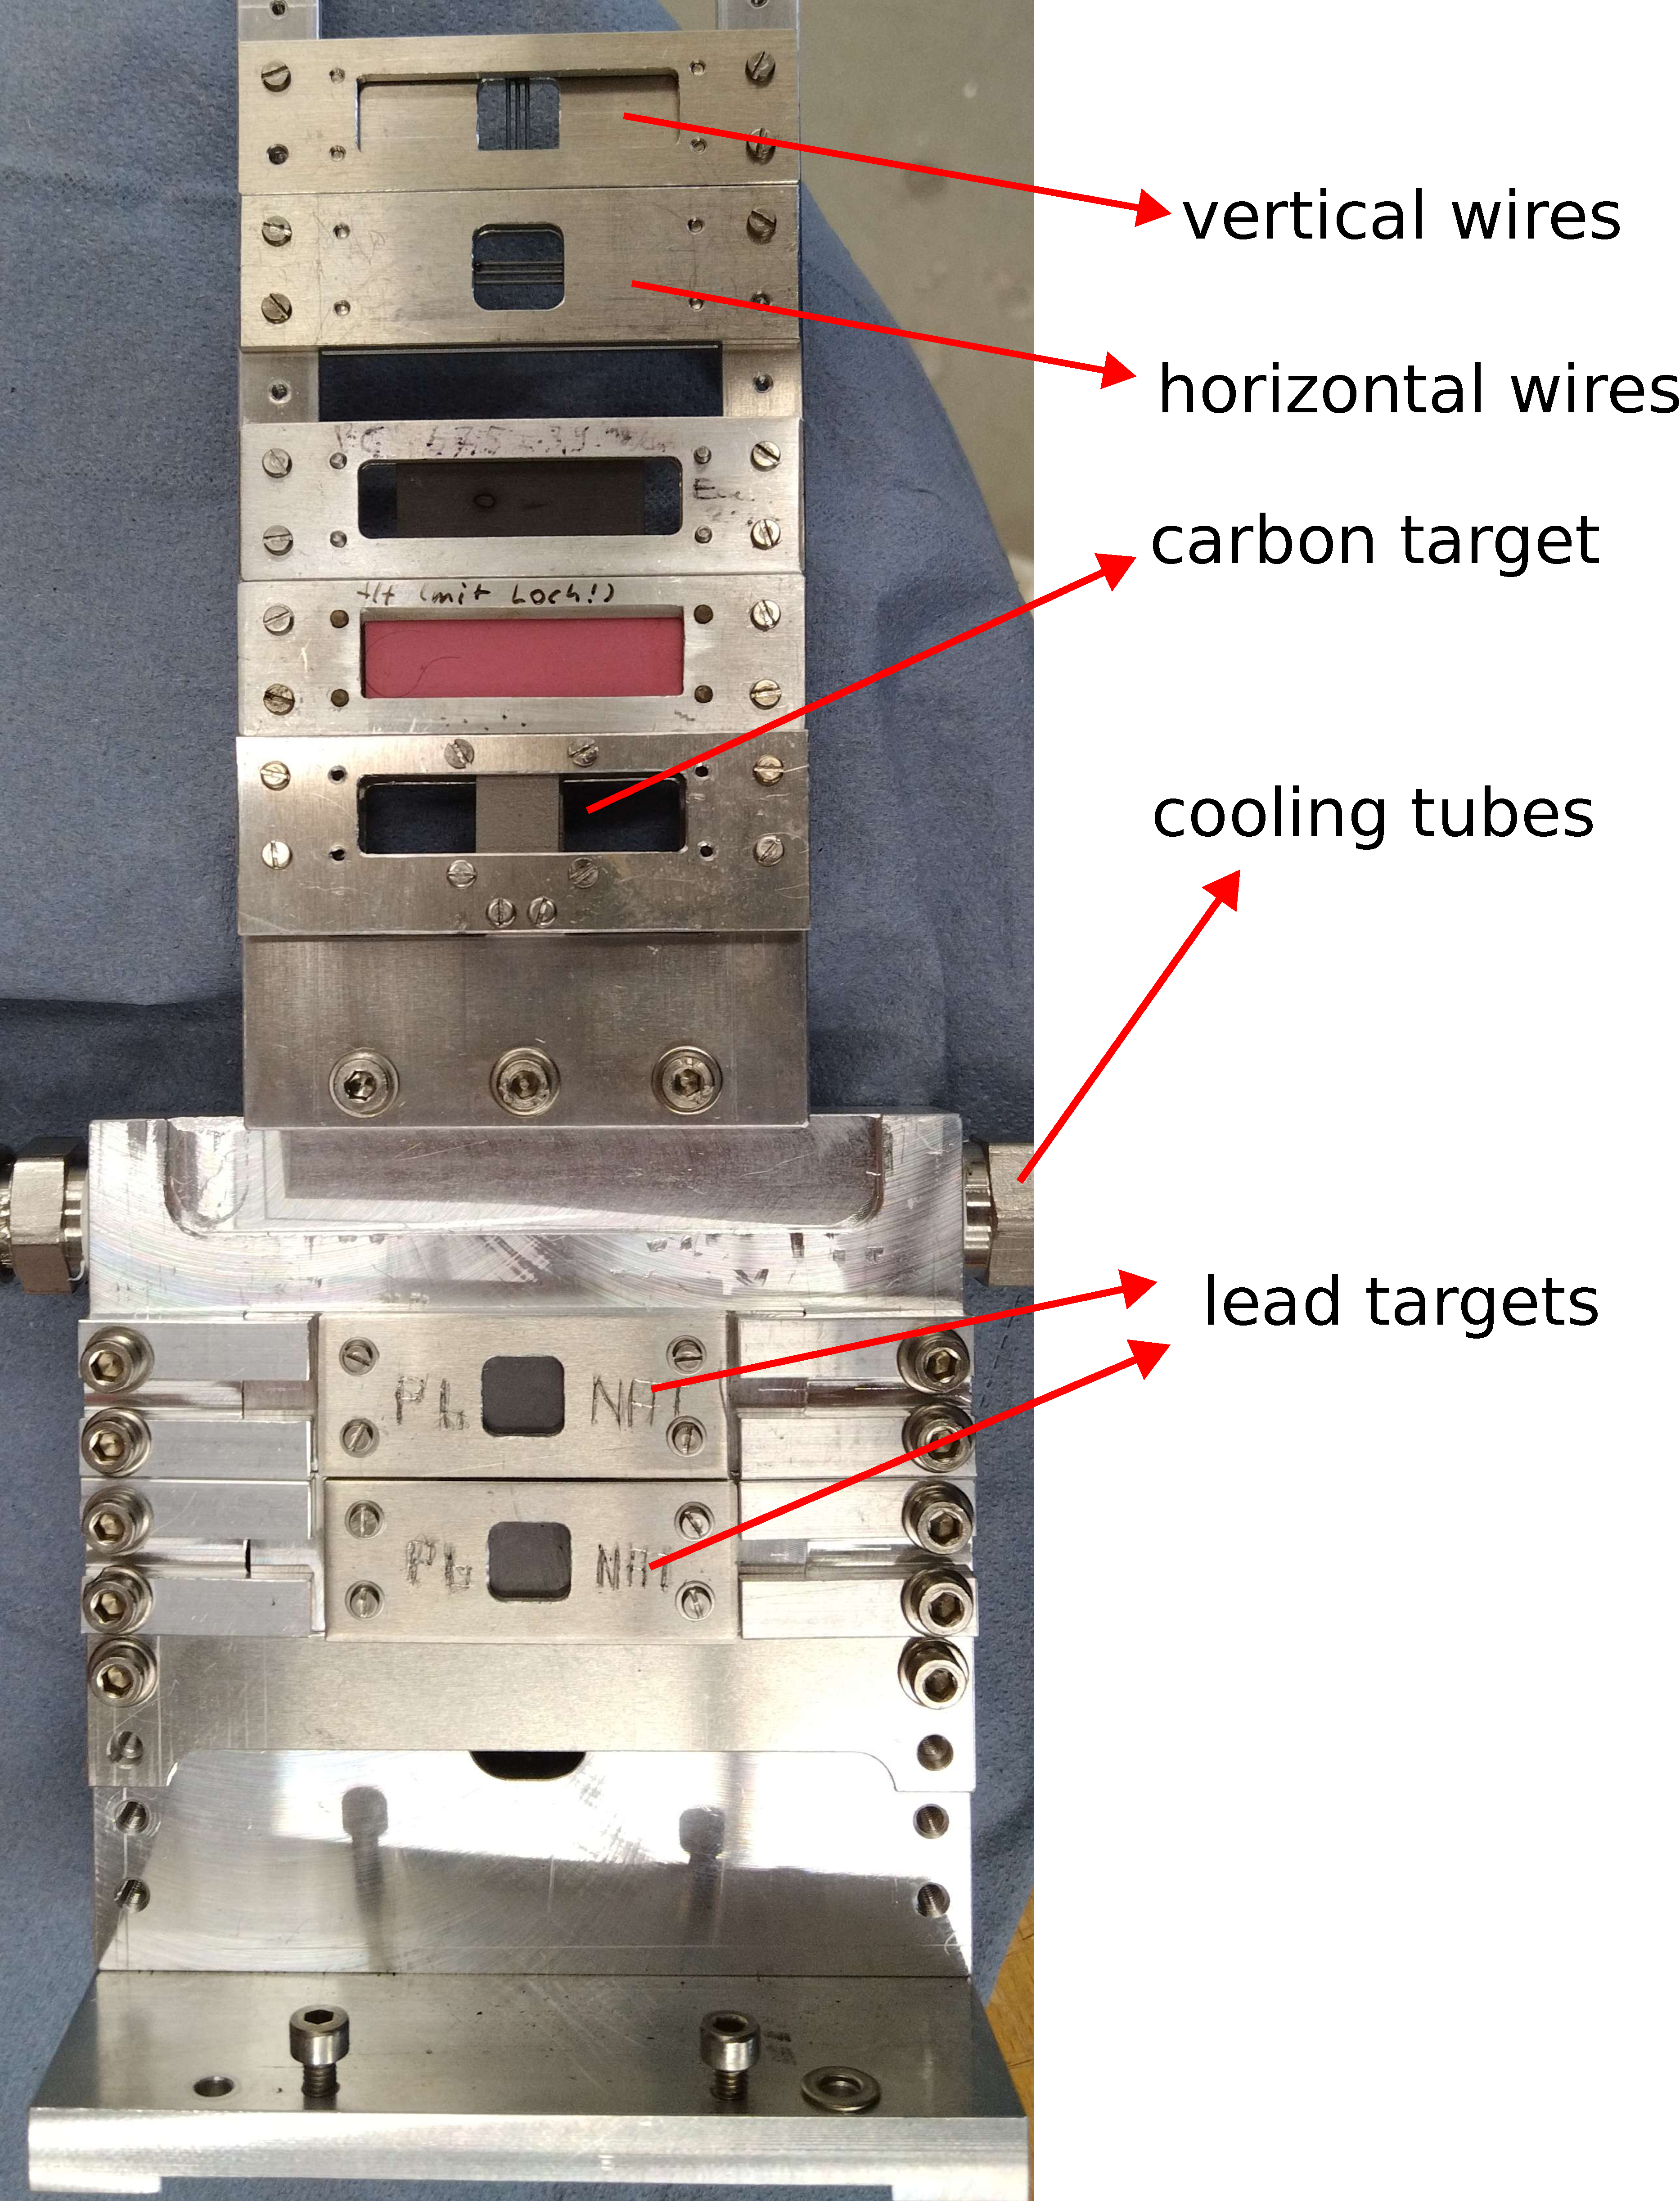
\includegraphics[width = 0.35\textwidth]{ExperimentalSetup/target.pdf}
\caption{Target frame installed during the experiment, on the top we have the two targets made by three carbon wires that are used to calibrate the positions monitors. Then the carbon target and the two lead targets.}
\end{wrapfigure}

 Then we repeat the same procedure with the other target, for the vertical direction. We observe that the pmts counts increase to a maximum, that is reached when the beam spot is centered on the carbon wire, and then decrease until the next carbon wire is hit by the beam.\\
We plot the pmt data \textit{versus} the $X25,X21,Y25,Y21$, given in $\SI{}{\volt}$. 
Given that we know the real distance between the two external wires, we can obtain the correct scaling factors to calculate the X and Y position values ​​of the beam. To identify the three peaks in of the carbon target, we fit the data using a gaussian model (see \ref{fig:HorizontalCalibration}). The mean $\mu$ represents the center of the wire, given in $\SI{}{\volt}$.

\begin{figure}[hbtp]
\centering
\includegraphics[scale=0.4]{figures/XYMOCalibBeamLine.svg.pdf}
\caption{Beam line scheme.}
\label{fig:BeamLine}
\end{figure}

Looking at the Beam line, we assume that the beam travels in a straight line. Let's consider the \textit{Wobbler 16} magnet the "$0$" of a coordinate system, with the $z$ axis pointing to the target (left direction in the beam scheme). The Beam parameters are measured by the Monitors $X/Y_{21}, X/Y_{25}$, which are located at some distance respect to the target. Suppose we are working only with the $Y_{25}$ monitor (the procedure is the same for the others). The Beam $y$ position is described by:

\begin{align*}
y_{beam} = m \cdot (z - z_{wobbler 16})
\end{align*}

In the scheme \ref{fig:BeamLine} we easily compute the distance between the $Y_{25}$ monitor and the \textit{wobbler 16} magnet, so we have the slope $m$. The Position on the target is given by $Y_{target} = m \cdot Z_{target}$. With these simple equations then:

\begin{equation}
c_{Y25} = \dfrac{d_{vertical} [\SI{}{\milli \meter}]}{ Y_{target}} 
\end{equation}

$c_{Y25}$ indicates the scaling factor of the monitor. With these values the Analysis program compute the correct beam position, and from that the incident angles in the $x,y$ directions, which are needed later for the analysis.

\begin{figure}[hbtp]
\centering
\includegraphics[width=0.4\textwidth]{Analysis/HorizontalCalibration.png}
\caption{•}
\label{fig:HorizontalCalibration}
\end{figure}

All this procedure can be easely checked if we plot now the $X$ and $Y$ position for the same two runs of data acquired with the wires. After placing the scaling factors obtained in the standard configuration file, we run the analysis another time and the physical values were computed \ref{fig:CheckHori}

\begin{figure}[hbtp]
\centering
\includegraphics[width=0.45\textwidth]{Analysis/XcheckB.png} 
\includegraphics[width=0.45\textwidth]{Analysis/XcheckA.png}
\caption{plot of the pmt Count against the physical values computed by the analysis program. Now the position of the three peaks correspond to the expected values measured for the target.}
\label{fig:CheckHori}
\end{figure}


\subsection{Current (PIMO) and energy monitors (ENMO) calibration.} \label{CurrentCalibration}

For the current monitors I13 and I21, we perform the calibration changing the current of the beam and observing the output values of the monitors (Voltage values). The we perform a fit (for the beam current, we used the nominal values that we communicate to MAMI, has the values for the x-axis).

\begin{figure}[hbtp]
\centering
\includegraphics[width = 0.45\textwidth]{Analysis/I13_Calibration.png}
\includegraphics[width = 0.45\textwidth]{Analysis/I21_Calibration.png} 
\caption{•}
\end{figure}

For the two monitors we are able to compute the offset and scale factor:

\begin{equation}
\begin{split}
I^{volt}_{13} = m_{13} \cdot I^{Nom}_{13} + q_{13}\\
c_{13} = \frac{1}{m} \qquad offset = -\frac{q_{13}}{m}
\end{split}
\end{equation}

The same formula for current monitor I21.

The Enmo calibration is performed in a different way from the other monitors. The polarity signal is sent to MAMI, and they produce a signal for the ENMO that somehow (need to investigate exactly how they do that) shows a difference between the first two subevents and the last two. This difference is equal (nominal) to $\SI{22.6}{\kilo \electronvolt}$. The idea now is to produce an histogram for the quantity $\delta E$ (with $E_{18}$ being the energy monitor):

\begin{equation*}
\delta E = \frac{E_{18}[2] + E_{18}[3]}{2} - \frac{E_{18}[0] + E_{18}[1]}{2} 
\end{equation*}

The data should be distributed with a peak around $\SI{22.6}{\kilo \electronvolt}$. To obtain the correct scaling factor for the values stored in the data tree we plot the voltage values mesured by the ENMO monitor.
3 runs of data where taken with different Beam current, to study the dependence of the measured quantity from the beam current. From the mean of the distribution it is possible to exstimate the scaling factor for the ENMO monitors, obtaining the physical quantity in the following way:

\begin{equation*}
C_{E18} = \frac{\SI{22.6}{\kilo \electronvolt}}{\overline{\delta E}}
\end{equation*}

\begin{figure}[hbtp]
\centering
\includegraphics[width = 0.45\textwidth]{Analysis/ENMOvoltage20.pdf}
\includegraphics[width = 0.45\textwidth]{Analysis/ENMOvoltage15.pdf} 
\caption{$\delta E$ for 20 $\SI{20}{\micro \ampere}$}
\end{figure}

Taking the average over $E_{18}$ voltage values, and using the formula above, we obtain the coefficient $C_{E18}$. To take care of the current depencende of the monitors, the scaling factor to be placed in the standard.config file is: $C_{E18} \overline{I}_{\mu A}$.
The calibration was performed taking three short acquisitions with different beam current : $\SI{20}{\micro \ampere}$, $\SI{15}{\micro \ampere}$ and a run without beam. 

\begin{figure}[hbtp]
\centering
\includegraphics[width = 0.5\textwidth]{Analysis/E18_Calibration.png}
\caption{Calibration of ENMO monitor}
\end{figure}

From this we obtain the value $scaling_{E18} = -1595.2$, to obtain the physical quantity from the analysis. As a final check the final histogram for the physical quantity is shown:

\begin{figure}[hbtp]
\centering
\includegraphics[width = 0.45\textwidth]{Analysis/ENMOCheck20.pdf}
\includegraphics[width = 0.45\textwidth]{Analysis/ENMOCheck15.pdf} 
\caption{Plot for the physical quantities computed in the data tree, for two different current of the beam (on the left $\SI{20}{\micro \ampere}$, $\SI{15}{\micro \ampere}$ on the right)}
\end{figure}



\subsection{Calibration of the pmts}

\commento{Here it's important to show the plots I made during the beam time. I have to mention the Leo tecniques for the correct interpretation of counts vs attenuation.}

During the beam time, several scans in attenuation were performed, before switching MAMI to produce the polarized beam, to choose the best working point for the PMTS of the detectors. The same procedure used in the laboratory was followed, starting from low attenuation and raising up the values. It's possible to get a simple model to describe the particular shape of the following plot taking into account simple assumptions about the type of electrical noise that affect the Nino board, and the \textit{pdf} of the signal produced by the PMTS.
The main assumption ("this is not a true assumption, Anselm has a plot of the digitalize charge that proves that") is that the signal amplitude, in $\SI{}{\milli \volt}$ collected by the Nino board is well described by a gaussian distribution, and for signal with low amplitude, we expect to be well described by an uniform distribution. Just to visualize, let's suppose that the distribution of the signal amplitude collected is of this type (\ref{fig:PDF}) (the following figure is just an example, the values ​​do not describe the data collected):

\begin{figure}[hbtp]
\centering
\includegraphics[width = 0.40\textwidth]{Analysis/distribution.pdf}
\caption{Example of the expected distribution of the PMTs output signal}
\label{fig:PDF}
\end{figure}

The probability for a signal to pass the selection is equal to the probability of being in above the threshold, that is the complementary cumulative of the gaussian distribution (probability of being in the right tail):

\begin{align*}
P(signal > thr) = 1 - \Phi(x) = \dfrac{1 - Erf(\dfrac{x_{thr} - x_{0}}{\sqrt{2} \sigma })}{2}
\end{align*}

Once we reach the uniform zone, the probability of an even being selected is proportional to the area of the rectangle, which increases linearly decreasing the threshold. Considering the normalization factor, it is straightfoward to fit the data with a model of this type:

\begin{equation}
\begin{split}
N(att) = N_{0} \cdot \dfrac{1 + Erf(\dfrac{x_{thr} - x_{0}}{\sqrt{2} \sigma })}{2} \qquad \text{if} \quad att < C  \\
N(att) = N(C) + m \cdot (att - C) \qquad \text{if} \quad att > C
\end{split}
\end{equation}

For the detector B we show the result assuming our model: 

\begin{figure}[hbtp]
\centering
\subfloat[][\emph{Attenuation scan for the pmts of detector B} \label{fig:AttScan}]
{\includegraphics[width = 0.75\textwidth]{Analysis/CalibrationPMT/Fit_attenuation.pdf}}
\end{figure}

\begin{figure}
\centering
\subfloat[][\emph{B0} \label{fig:Spectra}]
{\includegraphics[scale = 0.5]{Analysis/CalibrationPMT/B0.pdf}}
\subfloat[][\emph{B1}]
{\includegraphics[scale = 0.5]{Analysis/CalibrationPMT/B1.pdf}}\\
\subfloat[][\emph{B2}]
{\includegraphics[scale = 0.5]{Analysis/CalibrationPMT/B2.pdf}}
\caption{Recostructed spectra for Detector B, notice that we have \textit{Attenuation} values in the x axis, therefore right and left are swapped with respect to the graph \ref{fig:PDF}.}
\end{figure}

From the fit we obtain three valus for the signal Peak, given in attenuaton units.
We can check the idea behind this, visualizing the pmt count in a different way. Because we would like to visualize the number of electrons that generate a certain signal in the detector, we can think of differentiating the data showed in the plot \ref{fig:AttScan}. The differentiation consist in the difference between the Counts at a certain point and the previous one, and dividing by the increment in attenuation:

\begin{align*}
Spectra = \frac{N(att_{i}) - N(att_{i-1})}{att_{i} - att_{i-1}} 
\end{align*}

In this way we compute a discrete derivative of the plot showed in \ref{fig:AttScan}, which represent $\frac{\partial N}{\partial att}$. This is, in fact, the spectra of the signal, still given in attenuation units \ref{fig:Spectra}.\\
This plot are used to identify a good point to select the attenuation values. If we look at the plot (), we can see that the physical threshold does not scale linearly with changing the attenuation value, and for high values of attenuation, the threshold falls quickly at zero. Looking at the signal spectra, we indentify the first peak as the electron signal, and the other peak for higher attenuation values (on the right), correspond to very low threshold values, so it is noise that we want to reject. We select the values of the attenuation downstream ot the two distributions, taking all the pulses from the electron and rejecting rejecting most signal events. This is sufficient to carry out the calibration of the pmts. However, if we want to identify the physical threshold and want to obtain a plot of the spectra given in physical units, instead of attenuation unit, we can use a simple model to convert attenuation values to $\SI{}{\milli \volt}$:

\begin{align*}
f(att) = \dfrac{a}{(x - b)^{c} + d}
\end{align*} 

Specifical values of $a,b,c,d$ are suggested in the NINO board documentation. So the spectra values in physical units are represented by: 

\begin{figure}[h]
\centering
\subfloat[][]{\includegraphics[width = 0.45\textwidth]{Analysis/CalibrationPMT/voltB0.pdf} }
\subfloat[][]{\includegraphics[width = 0.45\textwidth]{Analysis/CalibrationPMT/voltB1.pdf} }\\
\subfloat[][]{\includegraphics[width = 0.45\textwidth ]{Analysis/CalibrationPMT/voltB2.pdf} }
\end{figure}

\newpage
\subsection{Autocalibration procedure} \label{Autocalib}

In this section we present the last calibration tecniques needed in the data-process. The autocalibration is a special operation mode of the MAMI accelerator, during which the beam current is made to vary in a controlled way. Through these special runs is possible to obtain again the current scaling factor that we discussed in \ref{CurrentCalibration}. Because the current in varying, it is possible to study the linearity of the pmts. From a linear fit of the pmts counts vs. current intensity the angular coefficient and the offset are measured. The offset is particual important because give rise of a possible systematic error that influence the final asymmetry result. It is quite simple to demostrate this, if a relation of the type $N = mI + N_{0} $ holds. Consider the following quantity:

\begin{align*}
\overline{N} = \frac{N_{\uparrow} + N_{\downarrow}}{2}
\end{align*} 

we can express $N_{\uparrow}$ and $N_{\downarrow}$ in this way:

\begin{align*}
N_{\uparrow} = \overline{N} + A_{n}\overline{N} \\
N_{\downarrow} = \overline{N} - A_{n}\overline{N} 
\end{align*}

Now we suppose that $\overline{N}$ is linear dependent on the current in the way we defined above, so:

\begin{align*}
N_{\uparrow} = \overline{N} + A_{n}(mI) + N_{0} \\
N_{\downarrow} = \overline{N} - A_{n}(mI) + N_{0} 
\end{align*}

We are supposing that the offset $N_{0}$, we assume that the present offset does not contribute to the asymmetry, i.e. it is not correlated to the signal of the scattered electrons, but is due to processes of another type, therefore in the previous formulas only the $mI$ counts must be multiplied by the asymmetry $A_{n}$. Therefore if we substitute everything in the definition of the transverse asymmetry:

\begin{equation} \label{eq:Systematic}
A^{'} = \dfrac{N_{\uparrow} - N{\downarrow}}{N_{\uparrow} + N{\downarrow}} = \dfrac{A_{n} (2mI)}{ (2mI) + 2N_{0} } = A_{n} \dfrac{1}{1 + \frac{N_{0}}{mI}}
\end{equation} 

In the last passage we learn that the presence of an offset can decrease the recostructed asymmetry. So it's important to determine quantitatively $N_{0}$ and $m$ in order to be able to take care of this effect. The strategy used is quite simple: every three hours of production data, we asked MAMI to start the autocalibration program. With all the autocalibration runs, we estimate $N_{0}$ for each pmt, separately. Then All this quantities are saved in a file so that the analysis program can retrieve the parameters and subtract them from the pmt counts. \medskip
In this way every three hours the pmt are corrected, this take care also of the possibility that the the linearity of the pmts can change after hours of use of the pmts (for example it can decrease the efficiency).

During the autocalibration, the beam current is raised from $\SI{9}{\micro \ampere}$ to $\SI{11.125}{\micro \ampere}$ in step of $\SI{0.125}{\micro \ampere}$: \newpage

\begin{figure}[ht]
\centering
\subfloat[][\emph{Autocalibration: in this plot we have the voltage value of I21 monitor. The current is first stabilized around $\SI{10}{\micro \ampere}$, then it is raised from $\SI{9}{\micro \ampere}$ (the step lower down) to $\SI{11.125}{\micro \ampere}$ in step of $\SI{0.125}{\micro \ampere}$.} \label{fig:Autocalibration}]{
\includegraphics[width = 0.75\textwidth]{Analysis/Autocalib/Current.pdf}}
\end{figure}

With a linear fit we can estimate the scale and the offset to convert from I21 voltage values to physical values of the current. The procedure in repeated for the $8$ autocalibration acquisition we had during the beam time, so we can also take care of possible variations during the time.

\begin{figure}[ht]
\centering
\subfloat[][\emph{Current scan for detector B, the error are multiplied by a factor of $20$.}]{
\includegraphics[width = 0.5\textwidth]{Analysis/Autocalib/fitB.pdf}} \\
\end{figure}

\begin{figure}[hbtp]
\centering
\subfloat[][\emph{Current scan for detector A, the error are \\ multiplied by a factor of $20$.}]{
\includegraphics[width = 0.49\textwidth]{Analysis/Autocalib/fitA0-3.pdf}}
\subfloat[][\emph{Current scan for detector A, the error are \\ multiplied by a factor of $20$.}]{
\includegraphics[width = 0.49\textwidth]{Analysis/Autocalib/fitA4-7.pdf}}
\caption{Pmt Rates vs current (from I21 monitor), the model used for the fit: $y = mx + q$.}
\end{figure}

\newpage
The figures are referred to the data acquired for the first autocalibration. It's interesting to calculate, from the result of the fit, the factor that appears in \ref{eq:Systematic}:

\begin{table}[ht]
\centering
\begin{tabular}{c|c|c|c}
\hline
 PMT & m [$\SI{}{\micro \ampere}^{-1}$] & Offset & c  \\
\hline
 B0  & 1750 &  1301 &  0.93 \\
 B1  & 1742 &  1283 &  0.93 \\
 B2  & 1406 &   717 &  0.95 \\
 A0  & 6423 & 20385 &  0.75 \\
 A1  & 6756 & 29187 &  0.70 \\
 A2  & 6032 & 20513 &  0.75 \\
 A3  & 5218 & 12995 &  0.80 \\
 A4  & 3945 &  6666 &  0.86 \\
 A5  & 3967 &  6547 &  0.86 \\
 A6  & 3258 &  4655 &  0.87 \\
 A7  & 2325 &  2233 &  0.91 \\
\hline
\end{tabular}
\end{table}
Ignoring the presence of the offset lead two consequences: the recostructed asymmetry is lower, on average $ \simeq 10\%$ less than expected, and the Counts are overstimated. Because the error depend on the pmt counts, as seen in \ref{eq:Error}, this two effect combined add up and worsen the precision and accuracy of the measurement.\\
The result reported in the table can be confronted with the final result that are reported in \ref{result}. 

\newpage



\chapter{Asymmetry on Carbon and Rates on Lead target.}

After having described all the calibrations needed, we are ready to analyze the data and measure the \transv from the data collected in second part of the beam time. In this chapter we explain the procedure for the pre-selection of the data (for example the removal of the events with large variation of the beam parameters) and the procedure used to analyze the recostructed asymmetry in order to obtain in the end a point exstimation for $A_{n}$. A section is dedicate to the measurement performed with lead target: the experimental rates measure using the detectors setup described here (\commento{mettere riferimento}) are reported; through the knowledge of the expected counts per sub-event, we calculate the amount of statistics needed to measure the \transv on $Pb$ with an accuracy of $1 ppm$. In the end we discuss the problem of the false asymmetries that can affect the final result, and also a raw exstimation of the systematic error is perfomed, in the end. 

\section{Rates on lead}

After all the calibrations are finally perfomed, the experimetal setup is ready to take real "production" data 
to achieve the objectives of the experiment. The first goal of the experiment is to measure the rates on $Pb$ target.
The lead target installed is a made by a thin layer with a thickness of $\SI{0.5}{\milli \meter}$, and it's not isotopically pure. The expected rates are given by the Mott cross section, that we report here \commento{mettere la sezione d'urto Mott, provare a fare i calcoli e vedere se torna}.\medskip

We took $14$ acquisitions lasting $\simeq 2,5$ minutes, which corresponds to $6950$ events. For each of these acquisitions we set the beam current at different values, ranging from $\SI{10}{\micro \ampere}$ to $\SI{22}{\micro \ampere}$ of intesity. The Rates are then reported as a function of the current, a linear model is used to fit the data.

\begin{figure}[hbtp]
\centering
\includegraphics[width = 0.9\textwidth]{Analysis/LeadRates/LeadRates.pdf}
\caption{Rates on lead Target in function of the beam current. The Rates for each PMT of detector A (on the left), and detector B (on the right) are reported.}
\end{figure}

The angular coefficient $m$ and the offset $q$ are reported in the table below. 

\begin{table}[ht]
\centering
\begin{tabular}{lllr}
\hline
 pmt   & m [\SI{}{\micro \ampere}]          & q                &  $\chi^{2}$ (dof = 9) \\
\hline
 A0    & 501.42 +/- 2.17 & 256.55 +/- 39.57 & 13.7521  \\
 A1    & 605.77 +/- 2.31 & 226.11 +/- 42.04 & 13.3783  \\
 A2    & 495.01 +/- 1.47 & 163.04 +/- 26.83 &  6.95713 \\
 A3    & 345.68 +/- 1.6  & 113.4 +/- 29.16  & 12.1727  \\
 A4    & 232.58 +/- 0.9  & 74.38 +/- 16.44  &  5.36892 \\
 A5    & 241.95 +/- 0.74 & 65.79 +/- 13.51  &  3.48398 \\
 A6    & 205.79 +/- 0.65 & 52.38 +/- 11.87  &  3.0892  \\
 A7    & 143.42 +/- 0.47 & 36.49 +/- 8.55   &  2.26341 \\
 B0    & 92.55 +/- 0.34  & -16.88 +/- 6.16  &  2.05286 \\
 B1    & 92.29 +/- 0.33  & -16.9 +/- 5.97   &  1.92163 \\
 B2    & 68.48 +/- 0.32  & -9.34 +/- 5.91   &  2.81988 \\
\hline
\end{tabular}
\end{table}

In this other plot we show the residuals: \commento{metti i residui, ma non sono poi coì interessanti da studiare}.

The pmt Counts with this target, increase from $100$ counts for detector B to $500$ counts every $\SI{1}{\micro \ampere}$.  The experimental error $\sigma$ related to the asymmetry was studied in \commento{aggiungi richiamo}, we recover the formula:

\begin{equation}
\sigma = \sqrt{\dfrac{1}{2 N \cdot n}}
\end{equation}

we remind to the reader that $N$ are the Counts per sub-event, while  $n$ is the number of event analyzed.
Now exstimate the amount of statistic needed to measure the asymmetry with some degree of accuracy. Let's suppose that we want to obtain, for each pmt, an error not greater than $4 ppm$. With this accuracy, the asymmetry obtained for detectro A will have an error given by $\frac{4ppm}{\sqrt{n_{pmt}}} \simeq 1.5 ppm$.
We computed the time needed to achieve this accuracy for both the two detectors, given in total hours of beam-time. To simplify the calculation, we assumed that every pmt rates of detector A and B are equal to the averaged counts obtained from the plot above.

\begin{table}[ht]
\centering
\begin{tabular}{c|c|c}
\hline
   current I &   T [h] Det A &   T [h] Det B \\
\hline
        10   &       344 &      1487  \\
        12.5 &       277 &      1185   \\
        15   &       232 &      985 \\
        17.5 &       199 &      843 \\
        20   &       175 &      737 \\
\hline
\end{tabular}
\end{table}

As we will see in the next part of this chapter, focused on the asymmetry on carbon target, the amount of time needed to obtain an accuracy of $\simeq 1.5 ppm$ is roughly $15 h$ with $\SI{10}{\micro \ampere}$. The same measurement with lead will need 23 times the statistic accumulated for Carbon. This involves more experimenta difficulties:

\begin{itemize}
\item deterioration of lead target.
\item need to develop a target cooling system.
\item monitor the radioactivity levels in the experimental hall.
\end{itemize}  
 
\section{Model for fitting the data}
\commento{Here I have to explain the model used for describing the data, so the problem of the false asymmetry induced by variations in beam position, angle, current and energy.}
\bigskip

One of the problems of the measurement is to take into consideration the various contributions that can change the value of the asymmetry measured by the experimental apparatus. The raw values of the asymmetry can be affected by the variation of the beam parameters during the time. Let's summarize quickly all these effects:
\begin{itemize}
\item the pmts counts  can depend on the $(x,y)$ impact position of the beam on the target
\item the variations of the incident angles $\theta_{x}$and $\theta_{y}$ on the target.
\item the uncertain associated with the energy of the Beam, a change in the energy associated with the polarization of the beam leads to different rates for the cross section
\item the uncertain associated with the current of the Beam, in particular a change due to the 
efficiency of the source in producing electrons polarized in the two opposite directions
\end{itemize}

All this quantity can influence the asymmetry measured by the pmts, considering also that the expected asymmetry is in the order of ten part per million, and small asymmetry introduced by fluctuations on the beam parameters are not negligible. Correcting directly the false asymmetries that rise from those uncertainties is a tough task, and it's more easy to adopt a different strategy respect to proceed to the analytical/numerical calculation of each of them . Knowing that the beam parameters produced by Mami are quite stable over the time, we can assume that the measured asymmetry are well described by a linear model as the following:

\begin{equation}
Asym = A_{physical} \cdot P + \delta_{I} + A_{x} \delta x + A_{y} \delta y + A_{\theta_{x}} \delta \theta_{x} + A_{\theta_{y}} \delta \theta_{y}+ A_{E} \delta E 
\end{equation}

$A_{physical}$ is the aim of the experiment, $A_{x}$ and $A_{y}$ are the asymmetries induced by the variation of the posizion of the beam, $A_{\theta_{x}}$ and $A_{\theta_{y}}$ are the asymmetry associated to angles, $A_{E}$ is the asymmetry associated to the beam energy. 
The relevant assumption is that, for small variation of the beam, the false asymmetry are linearly dependent on the Beam uncertainties (that are $\delta x, \delta y, \delta \theta_{x}, \delta \theta_{y}, delta_{E}$), so a first order approximation seems valid.\\
We must clarify now what we mean with $\delta x, \delta y, \delta \theta_{x}, \delta \theta_{y}, delta_{E}$. Resuming the event structure, that we discussed in \ref{FirstDescription}, we have a sequence of 4 different sub-events, with a polarization pattern that is randomly selected between $\uparrow,\downarrow,\downarrow, \uparrow$ and $\downarrow,\uparrow,\uparrow,\downarrow$. During the $\SI{20}{\milli \second}$ ot time lenght of each sub-event, the vfcs make a single measurement of the beam, and the data are saved in the data tree. The task of the analysis program is to use this raw data to calculate the relevant parameters for the analysis. Because we are working with asymmetries, the absolute values of the parameters listed above is not relevant, instead what is relevant are the differencies correlated with polarization state of the beam. Assuming this, $\delta x, \delta y, \delta \theta_{x}, \delta \theta_{y}, delta_{E}$ are replaced with :

\begin{equation}
\begin{split}
\delta {x} & = \Bigl(\dfrac{X_{\uparrow}(1) + X_{\uparrow}(2)}{2}\Bigl)  - \Bigl(\dfrac{X_{\downarrow}(1) + X_{\downarrow}(2)}{2}\Bigl)\\
\delta {y} & = \Bigl(\dfrac{Y_{\uparrow}(1) + Y_{\uparrow}(2)}{2}\Bigl)  - \Bigl(\dfrac{Y_{\downarrow}(1) + Y_{\downarrow}(2)}{2}\Bigl)\\
\delta {E} & = \Bigl(\dfrac{E_{\uparrow}(1) + E_{\uparrow}(2)}{2}\Bigl)  - \Bigl(\dfrac{E_{\downarrow}(1) + E_{\downarrow}(2)}{2}\Bigl)\\
\delta {\theta_{x}} & = \Bigl( \dfrac{\theta_{x,\uparrow}(1) + \theta_{x,\uparrow}(2)}{2} \Bigl) - \Bigl(\dfrac{\theta_{x,\downarrow}(1) + \theta_{x,\downarrow}(2)}{2} \Bigl)\\
\delta {\theta_{y}} & = \Bigl( \dfrac{\theta_{y,\uparrow}(1) + \theta_{y,\uparrow}(2)}{2} \Bigl) - \Bigl(\dfrac{\theta_{y,\downarrow}(1) + \theta_{y,\downarrow}(2)}{2} \Bigl)\\ 
\end{split}
\end{equation}

Each value represent the difference between the mean values over the two different polarization state.

\section{Data pre-selection and Fit}

After all the calibration are performed, the analysis program is ready to produce the datafiles suitable to analyze the asymmetry data for Carbon. \\
The Data file that are produced from the binary files are simply files in txt format, where the data are stored in columns. Before proceeding with the linear fit, however, it is necessary to visualize the data to check that there are no anomalous behaviors. In fact the data can contain moments of loss of the beam burrent and sudden interruptions, loss of polarization of the beam and even setting errors by MAMI operators can affect the experiment. Carbon data were taken from November 2nd to 4th, and consist of $28$ runs, each $1$ hour long.
The first step is to observe the pmt counts and the current trend, in order to be able to identify sudden interruptions of the beam. Here we show the trend over time for the series runs: 

\begin{figure}[hbtp]
\centering
\subfloat[][\emph{Pmt count trend versus time.In black A0, in green B0} \label{fig::CountTrend}]{
\includegraphics[width = 0.45\textwidth]{Analysis/Dataselection/BeamExample.pdf}}
\subfloat[][\emph{Asymmetry trend for pmt A0} \label{fig::AsymTrend}]{
\includegraphics[width = 0.45\textwidth]{Analysis/Dataselection/AsymmetryTrend.pdf}}
\end{figure}

This plot show that after 10 h of data acquisition the Pmt counts (\ref{fig::CountTrend}) dropped rapidly. If we show the current trend over the time (\ref{fig::CurrentTrend}) we do not see a corresponding decrease in beam intensity. Also the $x,y$ position (\ref{fig::PositionTrend}) and the energy monitor of the beam do not show a strange behavior. So we reject the possibility that at some point one of the stabilization device of the beam stop working. One of the possibilities is that something happen inside the two spectrometers. From the pmt counts we can suggest that the scattered electrons were not hitting our fused-silica detector,
in fact for pmt B0 we observe roughly 0 counts, and for pmt A0 $20000$ counts, which is compatible with the noisy offset of that pmt. This consideration strongly suggest as to reject those data from the analysis.\\
Apart from this, we observe in (\ref{analysis}) two steepy variations of the asymmetry around $13.5 h$ and $19 h$. For these data is quite simple to explain why should be rejected: we observe the same steepy variations also for the positions, so in this case the beam was not correctly aligned to the target.

\begin{figure}[hbtp]
\centering
\subfloat[][\emph{Current trend over time.} \label{fig::CurrentTrend}]{
\includegraphics[width = 0.45 \textwidth]{Analysis/Dataselection/CurrentTrend.pdf}}
\subfloat[][\emph{$X,Y$ beam position over time} \label{fig::PositionTrend}]{
\includegraphics[width = 0.45\textwidth]{Analysis/Dataselection/XYtrend.pdf} }
\end{figure}

After this first data selection, we check the correlated-difference data, which will be later used as variables for the fit. We produced histograms for all this quantites, that we remember are computed by the analysis program with the formula:

\begin{align*}
\delta x =  \frac{(x_{up,1} + x_{up,2})}{2} - \frac{(x_{down,1} + x_{down,2})}{2}
\end{align*}

We expect, if the stabilization of the beam is correctly set, that those quantities are gaussian distributed. A maximum likelihood fit with a Gaussian model is performed for each beam parameter, with Likelihood Ratio for the goodness of fit (gof). The statistic for the gof is:

\begin{align*}
\lambda(x) = 2 \sum_{i}^{n} (f_{i}(\mu) - k_{i}(1 + log(\frac{f_{i}(\mu)}{k_{i}})))
\end{align*}  

$\mu$ are the parameters of the \textit{pdf}, that are mean and variance of the gaussian, and $f_{i}(\mu)$ and $k_{i}$ are respectively the expected value for the i-nth bin and the observed value for the i-nth bin.

\newpage

\begin{figure}
\centering 
\subfloat[][\emph{$X$ position correlated difference}]{
\includegraphics[width = 0.3\textwidth]{Analysis/Dataselection/X.pdf}} 
\subfloat[][\emph{$Y$ position correlated difference}]{
\includegraphics[width = 0.3\textwidth]{Analysis/Dataselection/Y.pdf}}
\subfloat[][\emph{$\theta_{x}$ correlated difference}]{
\includegraphics[width = 0.3\textwidth]{Analysis/Dataselection/Xp.pdf}} \\
\subfloat[][\emph{$\theta_{y}$ correlated difference}]{
\includegraphics[width = 0.3\textwidth]{Analysis/Dataselection/Yp.pdf}}
\subfloat[][\emph{Energy correlated difference}]{
\includegraphics[width = 0.3\textwidth]{Analysis/Dataselection/ENMO.pdf}}
\end{figure}

Looking at the histograms, we see that the beam correlated-difference values are centered around zero, the result are reported below:

\begin{table}
\centering
\begin{tabular}{|c|c|c|c|c|c|}
\hline 
\rule[-1ex]{0pt}{2.5ex} & $X [\mu m]$ & $Y[\mu m]$ & $Xp [\mu rad]$ & $Yp [\mu rad]$ & $E [eV]$ \\ 
\hline 
\rule[-1ex]{0pt}{2.5ex} $\mu$ & $1.31 \cdot 10^{-3}$ & $2.4 \cdot 10^{-4}$ & $3.2 \cdot 10^{-8} $ & $3.6 \cdot 10^{-9}$ & $0.0013$ \\ 
\hline 
\rule[-1ex]{0pt}{2.5ex} $sigma$ & $3.7 \cdot 10^{-1}$ & $2.9 \cdot 10^{-2}$ & $ 1.9 \cdot 10^{-5} $ & $6.5 \cdot 10^{-6}$ & $0.38$ \\ 
\hline 
\end{tabular}
\label{parametri} 
\caption{Beam parameters}
\end{table}

these results are encouraging, the stabilization of the beam has meant that only small differences are observed within an event for each monitor. This means that, unless the values for the false asymmetries are not very large, the effect of the beam variation are small. we will have the opportunity to verify this hypothesis in the raw result. \bigskip
After removing the outliers, we mention a problem encountered during the data taking which took place on the night of the 2nd December. During that night the beam a wrong setting from the MAMI operators caused the beam to lose the polarization. We find out this problem only the next day, so we had not en evidence of how many hours of beam were lost. Unfortunatelly,  because this happened during the night, nobody could save the polarization measurement of the beam.
All the stabilization monitors were active, so the data show apparently the same behaviour of the good data taken during the first day of acquisition. We can't proceed with an arbitrary cut of the data, we risk to cut off also good data or perform an incomplete removal. However it's importat to indentify the data with this problem, ignoring this produce a overall measurement that is decrease respect to the theoretical prediction. This is the worst scenario, because we could not identify the presence, for example, of any other systematic effects related to the electronics system, therefore also the testing of the electronics is not possible.\\
 
The procedure to identify the runs with $0\%$ polarization rely to the exstimation of the correlation coefficient of the PMTs counts. \\
For every event we have two type of polarization sequence. The polarization $\vec{P}$ of each sub-event is identified with $+1$ and $-1$, that correspond to up and down $\overline{P}$. This values are part of the data tree, and form a sequence $p_{i}$ of the type: $+1-1-1+1,+1-1-1+1,-1+1+1-1$, where i is the index to the i-th sub-events analyzed. If the $\overline{P}$ is different from zero, we expect, due to the \transv, a difference in the number of scattered electrons between sub-events with different $p_{i}$. This lead to a positive/negative correlation between the sequence $p_{i}$ and the pmt data. In case of $\vec{P} = \vec{0}$, the expected values for the correlation should be zero. \\
We applied this strategy with the hope to identify and remove the block of data with $A_{n} \simeq 0$. The correlation $c$ coefficient between the $p_{i}$ and the pmt sequence $N_{i}$ of counts is computed every $t = 1 h$, that correspond to $45000$ events. We plot the averaged correlation for detector A and B, and the correlation of the two detectors together (with the reverse sign for detector B).

\begin{figure}[hbtp]
\centering
\subfloat[][]{
\includegraphics[width = 0.5\textwidth]{Analysis/Dataselection/Correlation.pdf}}
\subfloat[][]{
\includegraphics[width = 0.47\textwidth]{Analysis/Dataselection/OverallCorr.pdf}
}
\caption{Plot of the correlation fot the two detectors on the left, and the global correlation on the right. We clearly observe zero for a block of run starting at time $t = 12 h$, until $t = 19 h$.}
\end{figure}

This let us to identify the block of runs with the issues of $\vec{P} = \vec{0}$. It's important to double check that validity of this method seeing if the correspondi asymmetry is compatible with $0$. If we have these two evidences together, this confirms this last series of cuts. The asymmetries measured for suspicious runs are:

\begin{figure}[hbtp]
\centering
\includegraphics[width= 0.5\textwidth]{Analysis/Dataselection/Nopolarity.pdf}
\caption{•}
\end{figure}

This plot unequivocally shows that all the asymmetries measured for each PMTs for both detector A and B are compatible with zero. It is therefore reasonably certain that such data should not be included in the main analysis. However, this data is not useless. From them we can extract a reasonable estimate of possible systematic errors affecting our experimental setup. We report here the averaged asymmetries with the correspondig error for these runs:
\begin{itemize}
\item asymmetry $A =  -2.49 \pm 2.14$
\item asymmetry $B =  -7.83 \pm 6.50$
\end{itemize}

Even if every pmt is $1\sigma$ far from $A_{n} = 0$, the averaged values are negative and $2\sigma$ far from 0. This is an evidene of possible presence of a systematic effects.

Before proceeding with the fit, we observe how the asymmetry evolves as a function of time.

\begin{figure}[hbtp]
\centering
\includegraphics[width = 0.8 \textwidth]{Analysis/Dataselection/AveragedAsymmetry.pdf}
\caption{Plot of the Asymmetry versus time. For a point time $t_{1}$, we plot the mean over all the asymmetries collected from $t = 0$ to $t = t_{1}$. Each line represents the asymmetries measured for a specific pmt (in \textcolor{blue}{blue} detector B and in \textcolor{red}{red} detector A). The values are corrected for the beam polarization, multiplying by $\frac{1}{p}$. We plot also the error, which is one standard deviation $\sigma$ from the mean.}
\end{figure}

In this figure we plot the average of the asymmetries for each pmt, carried out from the beginning up to the instant $t$. The data shown are corrected with the percentage of polarization of the beam ($p \simeq = 0.79$). From this it can be seen how the asymmetry evolves as time increases. If there are still outliers data, we can directly check from this plot there a steepy variation in the data. 


When all the calibrations are performed, it is possible to proceed to generate the datafiles fot the fit program.
For a better visualization of the data, especially to observe the dependence of the asymmetry on the Beam parameters measured, it is useful to take the average asymmetry at regular intervals. From the raw plots of the asymmetries (see below \ref{fig:asyvsparam}), it is clear that the statistical error is too hight to identify a linear structure in the dependence of the asymmetry. 

\begin{figure}[hbtp]
\centering
\includegraphics[width = 0.5\textwidth]{Analysis/Asym_vs_monitor.png}
\caption{Asymmetries vs. Beam parameters}
\label{fig:asyvsparam}
\end{figure}

In all the figures the asymmetries are given in [ppm] units. The data are selected removing the correlated-difference that are $5\sigma$ far from the mean values, that we have reported in the table (\ref{parametri}) 

\begin{align*}
(x_{monitor} - \overline{x}_{monitor}) \leq 3 \cdot \sigma_{X}
\end{align*}

For each monitor we use the \textit{curve fit} function of the python library \text{scipy} to fit the data. Each Beam parameter is treated separately now, so in principle we are ignoring possible effect of correlation between the beam values. We are aware about this fact, the false asymmetries recostructed with this method can be affected by this bias. However this representation of the data offers a clear and understandable way to identify the presence of a linear structure in the data.

\newpage
\begin{figure}[hbtp]
\centering
\subfloat[][\emph{Asymmetries [ppm] vs X position [$mm$]}]
	{\includegraphics[width = 0.45\textwidth]{Analysis/clustering_XB.pdf}} \quad
\subfloat[][\emph{Asymmetries [ppm] vs Y position[$mm$]}]
	{\includegraphics[width = 0.45\textwidth]{Analysis/clustering_YB.pdf}} \\
\subfloat[][\emph{Asymmetries [ppm] vs $\theta_{x}$ angle [$rad$]}]
	{\includegraphics[width = 0.45\textwidth]{Analysis/clustering_XpB.pdf}} \quad
\subfloat[][\emph{Asymmetries [ppm] vs $\theta_{y}$ angle [$rad$]}]
	{\includegraphics[width = 0.45\textwidth]{Analysis/clustering_YpB.pdf}} \\
\subfloat[][\emph{Asymmetries [ppm] vs E [$keV$]}]
	{\includegraphics[width = 0.45\textwidth]{Analysis/clustering_EB.pdf}} \quad
\subfloat[][\emph{Asymmetries [ppm] vs I current [arb.unit]}]
	{\includegraphics[width = 0.45\textwidth]{Analysis/clustering_IB.pdf}} \quad
\label{fig:averageAsym}
\end{figure}

\begin{figure}[hbtp]
\centering
\subfloat[][\emph{Asymmetries [ppm] vs X position [$mm$]}]
	{\includegraphics[width = 0.45\textwidth]{Analysis/clustering_XA.pdf}} \quad
\subfloat[][\emph{Asymmetries [ppm] vs Y position[$mm$]}]
	{\includegraphics[width = 0.45\textwidth]{Analysis/clustering_YA.pdf}} \\
\subfloat[][\emph{Asymmetries [ppm] vs $\theta_{x}$ angle [$rad$]}]
	{\includegraphics[width = 0.45\textwidth]{Analysis/clustering_XpA.pdf}} \quad
%\subfloat[][\emph{Asymmetries [ppm] vs $\theta_{y}$ angle [$rad$]}]
%	{\includegraphics[width = 0.45\textwidth]{Analysis/clustering_YpB.pdf}} \\
%\subfloat[][\emph{Asymmetries [ppm] vs E [$keV$]}]
%	{\includegraphics[width = 0.45\textwidth]{Analysis/clustering_EB.pdf}} \quad
%\subfloat[][\emph{Asymmetries [ppm] vs I current [arb.unit]}]
%	{\includegraphics[width = 0.45\textwidth]{Analysis/clustering_IB.pdf}} \quad
\label{fig:averageAsym2}
\end{figure}


The error of each point is computed exploiting the same formula defined above (theory section; $N_{A/B}$ averaged pmt counts for each subevents and $n$ number of event in each interval):

\begin{align*}
\sigma_{Asym} = \dfrac{1}{\sqrt{2N_{A/B} \cdot n}}
\end{align*}


\section{False asymmetries}
\commento{Seems that is possible to obtain rough estimates of the beam related asymmetries with the results from the fit. For Energy and position it's achievable, while for the angles it's quite hard (in principle sounds possible to perform an analytic calculation of the asymmetry related to the incident beam angle, however Anselm told me that quite often those results are in disagrement with the observed even in the sign!).}

Until now the values for the false asymmetries were threated as the parameters of the fit. In this section we will investigate how we can obtain another different exstimations, usefult to check the validity of all the process of analysis of the data.

For $\frac{dA}{dX}$ and $\frac{dA}{dY}$, we conceptually exploit the possibility of varying the position of the beam on the target, as we did during one of the calibration phases. Using the same \textit{wobbler 16} we asked MAMI to slowly change the beam position on the X and Y monitor. The change in position has the effect to modify the rates for the two detector, and from them it's possible to extract exstimate the two false asymmetries related to the beam position. Now we will see how the two quantities are related.
From the plot .. we see that the counts are scaling linearly with the beam position, so we assume that the $N$ are given by

\begin{align*}
N(x,...) = N_{0} + m \cdot (x - x_{0})
\end{align*}

it is clear that the linear model can't be alwaws good, at some point the electron will be deflected completely out of the detector, and so the counts will fall rapidly to zero. However, the magnets used to deflect the beam are producing small variation in the position, on the order of hundredths of a millimeters.
Let's suppose that the beam position for two sub-events is $x_{1}$ and $x_{2}$, we can calculate the asymmetry between the two event, taking care of the possible effects due to the different position. We write explicitly: 

\begin{equation}
\begin{split}
Asym = \dfrac{N(x_{1}) - N(x_{2})}{N(x_{1}) + N(x_{2})} = \dfrac{N_{0} + m \cdot (x_{1} - x_{0}) - N_{0} - m \cdot (x_{2} - x_{0})}{N(x_{1}) + N(x_{2})} =  \dfrac{m}{2 N_{0} + m \cdot (x_{1} +  x_{2}) - 2m x_{0}}(x_{1} -  x_{2})
\end{split}
\end{equation}

In this equation three differents parameters appear: $N_{0}$ is the offset of the linear model, $m$ is the agular coefficient, or the slope, and $x_{0}$ is the initial position respect to we compute the position variation. The first two terms are obtained by a linear fit, while $x_{0}$ is fixed conveniently.

\begin{figure}[hbtp]
\centering
\subfloat[][\emph{Plot for slow variation in $x$ direction for detector B.}]
{\includegraphics[scale=0.5]{Analysis/slowxVariation.pdf}}
\subfloat[][\emph{Plot for slow variation in $x$ direction for detector B.}]{\includegraphics[scale=0.5]{Analysis/slowyVariation.pdf}}
\end{figure}


We can approximate the denominator deleting the term $ m \cdot (x_{1} +  x_{2})$ which should be small compared to $2N_{0}$. We end with:

\begin{equation}
Asym = \dfrac{m}{2N_{0} - 2mx_{0}}(x_{1} -  x_{2})
\end{equation}

The term in front of $(x_{1} - x_{2})$ can be compared to $\frac{dA}{dX}$. $x_{0}$ is arbitrary and can be set to 0. For $N_{0}$, the offset, we substitute the averaged value counts of each pmt for the polarized beam acquisitions ( we remind that the rate are collected during each $\SI{20}{\milli \second}$ time interval of each sub-event).\\
The data are reported in the table below:

\begin{center}
\begin{tabular}{|c|c|c|}
\hline 
Pmt & Detector A & Detector B \\ 
\hline 
pmt 0 & 84718 & 18925 \\ 
\hline 
pmt 1 & 96882 & 18815 \\ 
\hline 
pmt 2 & 80604 & 14807 \\ 
\hline 
pmt 3 & 65053 & \\ 
\hline 
pmt 4 & 45943 & \\ 
\hline 
pmt 5 & 46248 & \\ 
\hline 
pmt 6 & 37452 & \\ 
\hline 
pmt 7 & 25808 & \\ 
\hline 
\end{tabular} 
\end{center}
 
We report the values obtained with this new method ... 


We can investigate also the asymmetries related to the beam energy. For this one we can exploit the theoretical expression for the Mott cross-section, taking the derivative ...

We can investigate the Current asymmetries, because we have the autocalibration procedure, so from the scale factor we can check if the current asymmetri is compatible with $1$ as assumed or not.
\section{??Bootstrap??}

\commento{Although Anselm was against it, now seems possible to increase the precision of the mesurement with a procedure similar to a bootstrap. Instead of computing all the quantities inside a single event, it's possible to compute all the important quantities also between different events. In this scenario the statistics can be increased artificially as mutch as we want, with the same amount of data. Of course, it's also simple to abuse of this method, so we should restrict using only events next to each other. However seem reasonable and promising.}




